\chapter{Semi-parametric and non-parametric models}\label{chap11}

\section*{Solutions of Exercises}\label{sec11_1}
\begin{enumerate}[leftmargin=*]

\item Simulate a semi-parametric regression where  
\begin{align*}
	y_i &= 0.5x_{i1} - 1.2x_{i2} + \mu_i, \\
	p(\mu_i) &= 
	0.3 \phi(\mu_i \mid -0.5,0.5^2) + 0.7 \phi(\mu_i \mid 1,0.8^2).		
\end{align*}
Assume that $x_{i1}$ and $x_{i2}$ follow a standard normal distribution and that the sample size is 1,000. Perform inference in this model assuming that the number of components is unknown. Start with $H=5$ and use non-informative priors, setting $\alpha_{h0}=\delta_{h0}=0.01$, $\bm{\beta}_0=\bm{0}_2$, $\bm{B}_0=\bm{I}_2$, $\mu_{h0}=0$, $\sigma^2_{\mu 0}=10$, and $\bm{\alpha}_0=[1/H \ \dots \ 1/H]^{\top}$. Use 6,000 MCMC iterations, a burn-in period of 4,000, and a thinning parameter of 2. Compare the population parameters with the posterior estimates and plot the population density along with the posterior density estimate of $\bm{\mu}$ (the mean, and the 95\% credible interval).\\

\textbf{Answer}

We can see from the posterior estimates that three components disappear after the burn-in iterations. The 95\% credible intervals encompass the population values of all parameters, and the posterior density estimate closely matches the population density. See Figure \ref{figPMPDens}, where the black line represents the population density, the blue line denotes the posterior mean density estimate, and the shaded light blue area corresponds to the 95\% credible interval.
 
\begin{tcolorbox}[enhanced,width=4.67in,center upper,
	fontupper=\large\bfseries,drop shadow southwest,sharp corners]
	\textit{R code. Semi-parametric Gaussian mixture}
	\begin{VF}
		\begin{lstlisting}[language=R]
rm(list = ls()); set.seed(010101)
# Simulate data from a 2-component mixture model
n <- 1000
x1 <- rnorm(n); x2 <- rnorm(n)
B <- c(0.5, -1.2); X <- cbind(x1, x2)
z <- rbinom(n, 1, 0.3)  # Latent class indicator
mu <- ifelse(z == 0, rnorm(n, -0.5, 0.5), rnorm(n, 1, 0.8))
plot(density(mu))
y <- X%*%B + mu
# Hyperparameters
d0 <- 0.001; a0 <- 0.001
b0 <- rep(0, 2); B0 <- diag(2); B0i <- solve(B0)
mu0 <- 0; sig2mu0 <- 10
H <- 5; a0h <- rep(1/H, H)
# MCMC parameters
mcmc <- 2000
burnin <- 4000
tot <- mcmc + burnin
thin <- 2
# Gibbs sampling functions
PostSig2 <- function(Beta, muh, Xh, yh){
	Nh <- length(yh)
	an <- a0 + Nh
	dn <- d0 + t(yh - muh - Xh%*%Beta)%*%(yh - muh - Xh%*%Beta)
	sig2 <- invgamma::rinvgamma(1, shape = an/2, rate = dn/2)
	return(sig2)
}
PostBeta <- function(sig2, mu, X, y, Psi){
	XtX <- matrix(0, 2, 2)
	Xty <- matrix(0, 2, 1)
	Hs <- length(mu)
	for(h in 1:Hs){
		idh <- which(Psi == h)
		if(length(idh) == 1){
			Xh <- matrix(X[idh,], 1, 2)
			XtXh <- sig2[h]^(-1)*t(Xh)%*%Xh
			yh <- y[idh]
			Xtyh <- sig2[h]^(-1)*t(Xh)%*%(yh - mu[h])
		}else{
			Xh <- X[idh,]
			XtXh <- sig2[h]^(-1)*t(Xh)%*%Xh
			yh <- y[idh]
			Xtyh <- sig2[h]^(-1)*t(Xh)%*%(yh - mu[h])
		}
		XtX <- XtX + XtXh
		Xty <- Xty + Xtyh
	}
	Bn <- solve(B0i + XtX)
	bn <- Bn%*%(B0i%*%b0 + Xty)
	Beta <- MASS::mvrnorm(1, bn, Bn)
	return(Beta)
}
\end{lstlisting}
	\end{VF}
\end{tcolorbox} 

\begin{tcolorbox}[enhanced,width=4.67in,center upper,
	fontupper=\large\bfseries,drop shadow southwest,sharp corners]
	\textit{R code. Semi-parametric Gaussian mixture}
	\begin{VF}
		\begin{lstlisting}[language=R]
Postmu <- function(sig2h, Beta, Xh, yh){
	Nh <- length(yh)
	sig2mu <- (1/sig2mu0 + Nh/sig2h)^(-1)
	mun <- sig2mu*(mu0/sig2mu0 + sum((yh - Xh%*%Beta))/sig2h)
	mu <- rnorm(1, mun, sig2mu^0.5)
	return(mu)
}
PostBetas <- matrix(0, mcmc+burnin, 2)
PostPsi <- matrix(0, mcmc+burnin, n)
PostSigma2 <- list(); PostMu <- list()
PostLambda <- list(); Reg <- lm(y ~ X)
Beta <- Reg$coefficients[2:3]; Res <- Reg$residuals
plot(density(Res))
Resq <- quantile(Res, c(0.2, 0.4, 0.6, 0.8))
Id1 <- which(Res <= Resq[1])
Id2 <- which(Res > Resq[1] & Res <= Resq[2])
Id3 <- which(Res > Resq[2] & Res <= Resq[3])
Id4 <- which(Res > Resq[3] & Res <= Resq[4])
Id5 <- which(Res > Resq[4])
Nh <- rep(n/H, H); Lambda <- rep(1/H, H)
MU <- c(mean(Res[Id1]), mean(Res[Id2]), mean(Res[Id3]), mean(Res[Id4]), mean(Res[Id5]))
Sig2 <- c(var(Res[Id1]), var(Res[Id2]), var(Res[Id3]), var(Res[Id4]), var(Res[Id5]))
Psi <- rep(NA, n); Hs <- length(MU)
pb <- winProgressBar(title = "progress bar", min = 0, max = tot, width = 300)
for(s in 1:tot){
	for(i in 1:n){
		lambdai <- NULL
		for(h in 1:Hs){
			lambdaih <- Lambda[h]*dnorm(y[i] - X[i,]%*%Beta, MU[h], Sig2[h]^0.5)
			lambdai <- c(lambdai, lambdaih)
		}
		Psi[i] <- sample(1:Hs, 1, prob = lambdai)
	}
	PostPsi[s, ] <- Psi
	Hs <- length(table(Psi))
	for(h in 1:Hs){
		idh <- which(Psi == h)
		Sig2[h] <- PostSig2(Beta = Beta, muh = MU[h], Xh = X[idh,], yh = y[idh])
		MU[h] <- Postmu(sig2h = Sig2[h], Beta = Beta, Xh = X[idh,], yh = y[idh])
	}
	PostSigma2[[s]] <- Sig2
	PostMu[[s]] <- MU 
	Beta <- PostBeta(sig2 = Sig2, mu = MU, X = X, y = y, Psi = Psi)
	PostBetas[s,] <- Beta
	Lambda <- sort(MCMCpack::rdirichlet(1, a0h[1:Hs] + table(Psi)), decreasing = TRUE)
	PostLambda[[s]] <- Lambda
	setWinProgressBar(pb, s, title=paste( round(s/tot*100, 0),"% done"))
}
close(pb)
\end{lstlisting}
	\end{VF}
\end{tcolorbox}

\begin{tcolorbox}[enhanced,width=4.67in,center upper,
	fontupper=\large\bfseries,drop shadow southwest,sharp corners]
	\textit{R code. Semi-parametric Gaussian mixture}
	\begin{VF}
		\begin{lstlisting}[language=R]
keep <- seq(burnin, tot, thin)
PosteriorBetas <- coda::mcmc(PostBetas[keep,])
summary(PosteriorBetas); plot(PosteriorBetas)
PosteriorPsi <- PostPsi[keep,]
Clusters <- sapply(1:length(keep), function(i){length(table(PosteriorPsi[i,]))})
PosteriorSIGMA <- matrix(NA, length(keep), 2)
PosteriorMU <- matrix(NA, length(keep), 2)
PosteriorLAMBDA <- matrix(NA, length(keep), 2)
l <- 1
for (s in keep){
	PosteriorSIGMA[l,] <- PostSigma2[[s]][1:2]
	PosteriorMU[l,] <- PostMu[[s]][1:2]
	PosteriorLAMBDA[l,] <- PostLambda[[s]][1:2]
	l <- l + 1
}
summary(coda::mcmc(PosteriorSIGMA))
summary(coda::mcmc(PosteriorMU))
summary(coda::mcmc(PosteriorLAMBDA))
# Posterior density estimate #
mus <- seq(-3, 4, 0.01)
DensityEst <- function(par, eval){
	lambda1 <- par[1]; lambda2 <- par[2]
	mu1 <- par[3]; mu2 <- par[4]
	sd1 <- par[5]; sd2 <- par[6]
	Dens <- lambda1 * dnorm(eval, mu1, sd1) + lambda2 * dnorm(eval, mu2, sd2)
	return(Dens)
}
par <- cbind(PosteriorLAMBDA, PosteriorMU, PosteriorSIGMA^0.5)
DensEval <- matrix(NA, length(keep), length(mus))
DensPop <- rep(NA, length(mus))
for(r in 1:length(mus)){
	for(l in 1:length(keep)){
		DensEval[l, r] <- DensityEst(par = par[l,], eval = mus[r])
	}
	DensPop[r] <- DensityEst(par = c(0.7, 0.3, -0.5, 1, 0.5, 0.8), eval = mus[r]) 
}
library(dplyr); library(ggplot2); require(latex2exp)
DataDens <- tibble(t = mus, Pop = DensPop, lower = apply(DensEval, 2, quantile, probs = 0.025), upper = apply(DensEval, 2, quantile, probs = 0.975), meanT = colMeans(DensEval))
plot_filtering_estimates <- function(df) {
	p <- ggplot(data = df, aes(x = t)) + 	geom_ribbon(aes(ymin = lower, ymax = upper), alpha = 1, fill = "lightblue") + 	geom_line(aes(y = Pop, color = "True Value"), linewidth = 0.5) + 	geom_line(aes(y = meanT, color = "Estimate"), linewidth = 0.5) +
	scale_color_manual(values = c("True Value" = "black", "Estimate" = "blue")) + xlab(TeX("$\\mu$")) + ylab("Density") + 	labs(title = "Density: Stochastic Errors", color = "") + theme_minimal()
	print(p)
}
plot_filtering_estimates(DataDens)
\end{lstlisting}
	\end{VF}
\end{tcolorbox}

\begin{figure}[!h]
	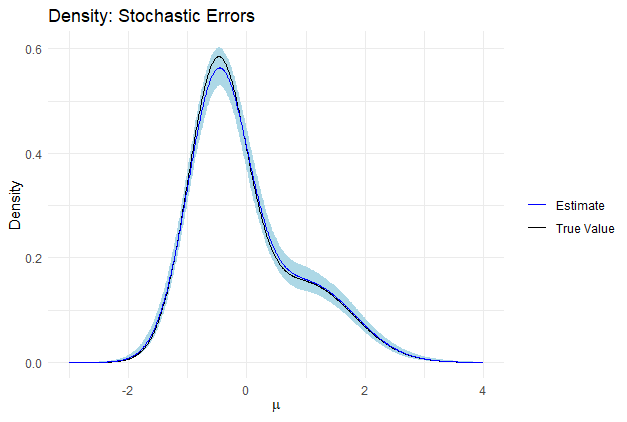
\includegraphics[width=340pt, height=200pt]{Chapters/chapter11/figures/DensEstSE.png}
	\caption[List of figure caption goes here]{Posterior density estimate: Stochastic errors.}\label{figPMPDens}
\end{figure}
 
\end{enumerate}